\chapter{Trabajo Previo}
 En este capítulo, se resumen los alcances del proyecto mesa de ayuda iniciado por Pablo Arancibia y acogido por el \acrshort{cadcc}. Se divide en los detalles relevantes de la solución existente y los alcances de esta plataforma.
\section{Solución existente}
    El proyecto iniciado el 2020, cuanta esencialmente con un diseño basado en una arquitectura de 4 partes: Database, back-end, aplicación web y el bot. El Modelo de datos se basa principalmente en la información que el sistema consume, credenciales de usuarios y feedback de los usuarios de bot. Este sistema es una gran mejora a las vías actuales de información de los alumnos, principalmente porque está diseñado para responder las dudas de los estudiantes de manera satisfactoria, mejora la comunicación entre alumnos y funcionarios, además de estar validado por la comunidad del dcc \cite{ARANCIBIA2021}.

    \subsection{Arquitectura Previa}
        \begin{figure}[h]
            \centering
            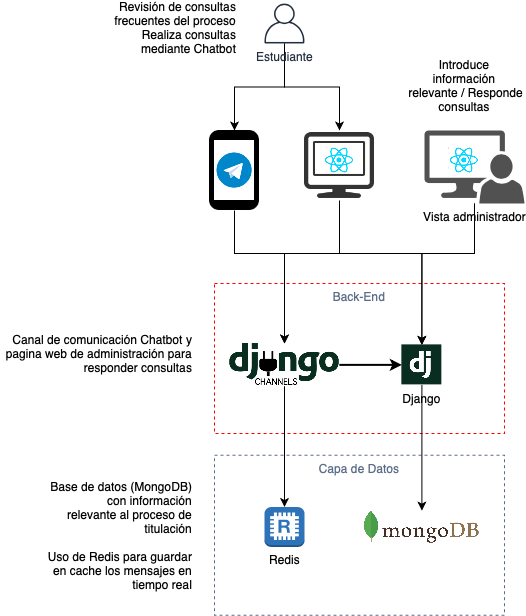
\includegraphics[scale=0.5]{media/imagenes/trabajo_previo/arquitectura_del_sistema.png}
            \caption[Arquitectura sistema anterior]{Esquema de arquitectura del trabajo realizado por Pablo Arancibia. Obtenido desde \cite{ARANCIBIA2021}}
            \label{fig:arc-previa}
        \end{figure}

        \par Cómo se puede observar en la figura \ref{fig:arc-previa}, la capa de datos cuenta con dos bases de datos: Redis y Mongodb. Redis se usa para guardar mensajes en caché en tiempo real, enviados por ejemplo desde un estudiante a través del bot a un asistente en la plataforma de administración web. Mientras que Mongo se usa para almacenar la información relevante de los procesos, las cuentas de los usuarios, los mensajes de los usuarios de forma persistente, etc.
        \par El back-end hecho en Django, sirve tanto al bot, la plataforma web de estudiantes y administración. Aquí se utiliza la tecnología de django channels para sincronizar mensajes desde el bot a la vista web. django principalmente se usa para manejar las consultas a la base de datos por información, cómo el procesamiento y traspaso de mensajes desde el bot.
        \par El front por otra parte se divide entre la plataforma de telegram y el front diseñado en react, para la vista de alumnos y administración. El Bot utiliza la API de \gls{Telegram} para genera vistas e interactuar con el usuario. La plataforma web por otra parte es una aplicación completa que muestra información sobre el proceso además de proveer el módulo de administración, para contestar mensajes, editar la información, entre otras.

    \subsection{Modelo de Datos Previo}
        \begin{figure}[h]
            \centering
            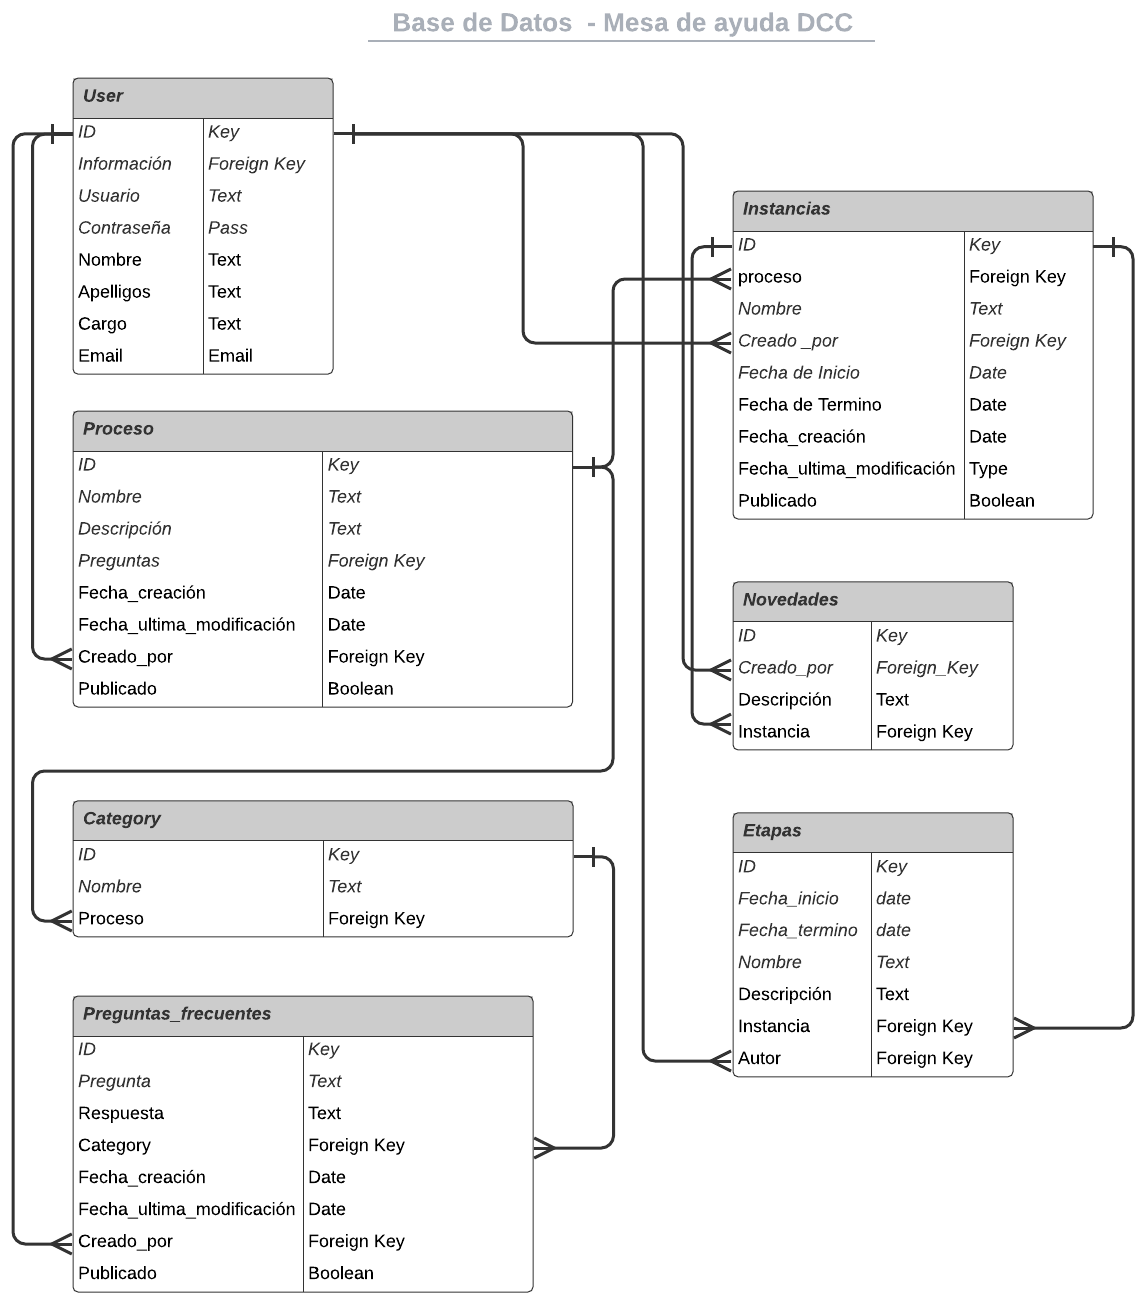
\includegraphics[scale=0.25]{media/imagenes/trabajo_previo/modelo_datos.png}
            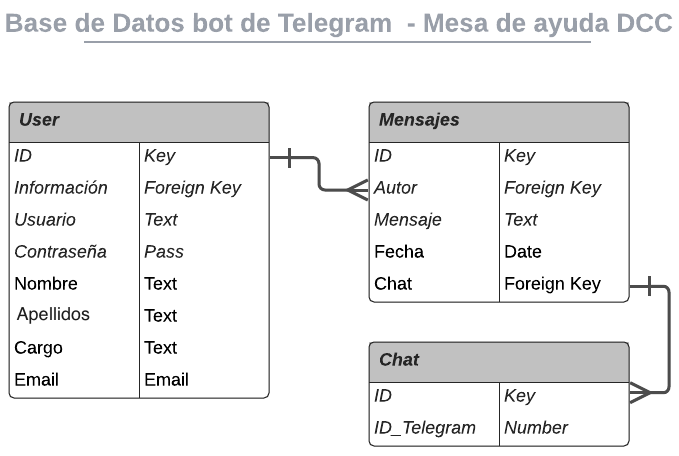
\includegraphics[scale=0.25]{media/imagenes/trabajo_previo/modelo_datos_bot.png}
            \caption[Modelo de datos]{Modelo de datos del trabajo realizado por Pablo Arancibia. Obtenido desde \cite{ARANCIBIA2021}}
            \label{fig:md-previo}
        \end{figure}
        
        \par El modelo de datos se puede estudiar en detalle en \cite{ARANCIBIA2021}, pero a grandes rasgos. Tiene las credenciales de los usuarios de administración \footnote{tabla user} y la información de los procesos.
        \par La información de los procesos académicos, esta distribuida en 2 grandes áreas, aquella que es semi estática\footnote{Se dice semi estática y no completamente estática, porque la información en la base se puede modificar, sin embargo, es transversal a la fecha de consulta o de realización de un proceso.} en el tiempo y la que cambia continuamente. 
        \par La información relacionada con un proceso, cómo por ejemplo \guillemotleft Proceso de Titulación \guillemotright o \guillemotleft prácticas profesionales \guillemotright es el nombre, la descripción, las preguntas frecuentes y las categorías de estas preguntas frecuentes. Por otro lado, una instancia del proceso, cómo por ejemplo  \guillemotleft Proceso de Titulación 2022 \guillemotright, tiene asociadas las novedades y las etapas de dicho proceso, ya que estas van a variar de instancia a instancia.

    \subsection{Módulos lógicos del bot}
        \begin{figure}[h!]
            \centering
            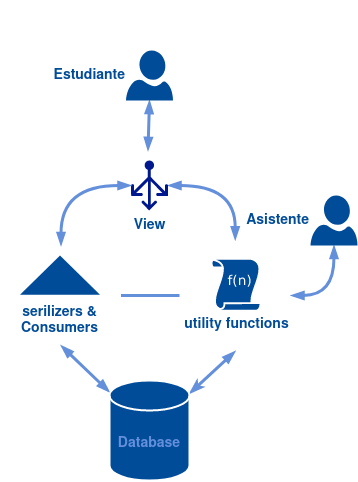
\includegraphics[scale=0.5]{media/imagenes/trabajo_previo/Bot_Modules-old.png}
            \caption[Funcionamiento del Bot]{Diagrama que esquematiza el funcionamiento del bot.}
            \label{fig:bot-work-old}
        \end{figure}
        \par la aplicación del bot, actualmente cuenta con los scripts default de Django más routing utilziado por django channels, además de \textit{consumers} y \textit{serializers} que se usan para seguir un estándar \gls{REST}.
        \par los \textit{scripts consumers} y textit{serializers} engloban la lógica de serializar los datos y procesar las \textit{requests} y la data anexa de json para traducirlas a \gls{Django}. Por otra parte routing es utilizado en caso de que sea necesario establecer un websocket entre la aplicación web y el servidor para mantener una comunicación en tiempo real entre el administrador y el alumno.
        \par en el modulo view, se hace el procesamiento de los \textit{requests}, actualmente engloba la mayoria de las operaciones y funciones del bot como eviar mensajes, procesar input del usuario, extraer data para el chat desde la base de datos y guardar inputs en ella.

    \subsection{Problemas del trabajo previo}
        \subsubsection{Falta de modularización}
            \par El bot, cómo estaba desarrollado, incluía la mayoría de las funciones nucleares en la \textit{view} de \gls{Django} (ver \ref{list:view}). Esto implica que no es claro dónde se podría modificar el código para agregar nuevas funcionalidades. Si se desea mantener el diseño, la única forma de extender el código es añadiendo nuevas funciones o modificando las existentes, sin mejorar el orden lógico. Esto tácitamente implica que para cada cambio grande se debe hacer un \textit{refactoring} del código actual. Además lo hace poco legible, hace que trabajar simultáneamente en el proyecto implique hacer \textit{brach} y \textit{merges} en un sistema de versionamiento por ejemplo, a pesar de que dos personas trabajen en áreas similares. Estas deficiencias hacen que el proyecto no sea escalable, no por arquitectura física o capacidades del sistema, sino porque no porque la única forma de lograr extender el sistema de forma ordenda y manteniendo la integridad del mismo, es modificar la disposición del código existente. 
            
        \subsubsection{Ausencia de delegación de responsabilidades}
            \par Ya que la mayoría de las funcionalidades del bot, se encuentran todas bajo el mismo \textit{script} y además bajo el \textit{scope} de la función principal de la view. La única forma de procesar distintos protocolos de comunicación o formas de procesar mensajes, es través de condicionales sobre el contenido del código, esto implica que la ramificación y extensión de la función principal puede crecer indefinidamente a medida que se deseen agregar nuevas formas de entendimiento, cómo comandos de telegram o procesamiento de lenguaje natural.
            \par También implica que la lógica de acción a realizar depende de la misma capa en el sistema, por lo tanto, al ir añadiendo funcionalidades se crea una sobrecarga sobre esta parte de la API. Asi mismo resulta difícil agregar nuevos comportamientos sin extender el código existente, lo que hace aún menos claro cómo funciona el procesamiento de mensajes.
        \subsubsection{Ausencia de Documentación}
            \par El sistema actual solo cuenta con un \textit{README}, que tiene la información esencial para ejecutar el proyecto. Pero hay nula información sobre cómo funciona el sistema, sobre cómo se pueden extender los módulos actuales, cómo se comunican las diferentes partes del sistema. Esto hace que el proyecto dependa de que las personas que trabajan en él, deban conocerse y comunicarse continuamente. En el caso de perder esta comunicación el proyecto queda virtualmente desechado, porque la configuración es lo suficientemente compleja, como para hacer difícil que alguien la tome y la extienda sin apoyo de un desarrollador del proyecto. 
            \par Por otro lado muchas de las librerías utilizadas en el sistema están bajo cambios constantes, al punto de que durante el trabajo de esta memoria cambiaron su comportamiento, incluso la documentación de lugar. Algunas se volvieron proyectos con una versión de pago, y eso hace que si alguien que no conoce estas librerías toma el proyecto, le tomará un tiempo largo entender los errores que el sistema puede arrojar. Incluso, pueden iniciarse errores inesperados o \textit{dataraces}, lo que harían al sistema inutilizable. 
            \par Cómo uno de los objetivos es que este sistema sea adoptado por los estudiantes del departamento y extendido por ellos, estas faltas de documentación no pueden existir, porque este material es necesario para mantener, extender y mejorar el proyecto.
            \par Finalmente, las tecnologías utilizadas son variadas y diversas, por lo tanto para alguien no familiarizado con ellas, tienen una curva de aprendizaje media alta. Cada una de estas herramientas es extensa tanto en funcionalidades como en documentación, por lo tanto, esto sumado a los cambios constantes, hacen que el proyecto no sea extensible por terceros.

            \begin{listing}
                \begin{minted}{python}
                    class BotView(View):
                        def post(self, request, *args, **kwargs):
                            try: # access field chat_id
                            except Exception as e:
                            try:# access field label
                            self.message_processing(...)
                            return JsonResponse({"ok": "POST request processed"})
        
                        def message_processing(...):
                            messages = []
                            if label is None:
                            if message == '/start': messages = # [list of messages]
                            elif message == '/preguntasFrecuentes':
                            else: # contactar a un asistente
                            elif label == 'Process':  # [list of messages]
                            elif label == 'Category':  # [list of messages]
                            elif label == 'Question':  # [list of messages]
                            elif label == 'Feedback':  # [list of messages]
                            elif label == 'Helper':  # [list of messages]
                            for msg in messages:
                            self.send_message(msg['text'], t_chat["id"], msg['keyboard'])
        
                        # all functions below are static functions
                        def get_process_keyboard():
                        def get_name_process(id):
                        # Similar for category, other functions
                        def send_message_website(message, t_chat):
                        def send_message(message, chat_id, keyboard_button={}):
                    
                \end{minted}
                 \caption[View sistema anterior]{Resumen del código contenido en la \textit{View} de \gls{Django}}
                 \label{list:view}
            \end{listing}
        

\section{Alcances de la solución existente}
    \par Durante la finalización del trabajo anterior, el trabajo con \acrlong{f}, y en conversaciones con el \acrlong{cadcc}. Los estudiantes se han visto favorables a adoptar la plataforma \cite{ARANCIBIA2021}. Han habido varios comentarios acerca de las funcionalidades que debiera incluir, que mejoras se les podría hacer, pero en general se podría decir que la solución tendría una aceptación tal cual esta, solo que aún le faltarían funcionalidades para reemplazar la mayoría de los otros canales de información.
    \par Si bien la solución existente es viable, aún no ha sido puesta en producción de forma definitiva, aunque está disponible en una versión de desarrollo por el \acrshort{cadcc}.
    
